\documentclass[../main.tex]{subfiles}

\begin{document}
\chapter{Konstruktion der Reellen Zahlen}
\section{Historische Motivation}
In der Antike war Mathematik praktisch synonym mit Geometrie. Der Zahlenbegriff war
direkt an das Konzept der \textit{Länge} gekoppelt.

\begin{definition}[Euklid, 300 vor Christus]
  Zwei Längen $a,b > 0$ heissen \textit{kommensurabel}, falls eine Länge $L>0$ existiert,
  so wie zwei natürliche Zahlen $m,n \in \mathbb N$, so dass $a = mL$ und $b=nL$.
\end{definition}

Hier ist
\[\mathbb N = \{0, 1, 2, 3, 4, \dots\}\]
die Menge der Natürlichen Zahlen.

\begin{theorem}[Euklid]
  Die Seite und Diagonale eines ebenen Quadrats sind nicht kommensurabel.
\end{theorem}

\begin{proof}
  Dieser Beweis ist geometrisch, nach Euklid. Wir nehmen an, es gäbe $L > 0$ und
  $m,n \in \mathbb N$ mit $x = mL$ und $d = nL$. Wir zeigen, dass das zu einem Widerspruch
  führt.
  Wir stellen fest, dass die Längen $x_{1} = d-x$ und $d_{1} = 2x - d$
  ebenfalls die Seite und Diagonale eines Quadrats bilden, siehe Abbildung
  \ref{fig:euklid}.

  \begin{figure}[htb]
    \centering
    \begin{minipage}{0.4\linewidth}
      \centering
      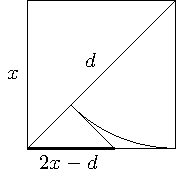
\includegraphics{images/euklid-quadrat}
    \end{minipage}%
    \begin{minipage}{0.4\linewidth}
      \centering
      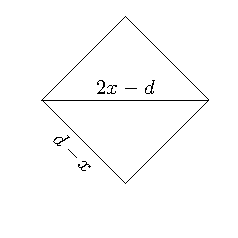
\includegraphics{images/euklid-quadrat2}
    \end{minipage}
    \caption{Euklids Konstruktoin}%
    \label{fig:euklid}
  \end{figure}

  Weiterhin gilt, dass sowohl $x_{1}$ als auch $d_{1}$, ganze Vielfache von $L$ sind:
  \begin{align*}
    x_{1} = d-x = (n-m)L \\
    d_{1} = 2x-d = (2m -n)L
  \end{align*}
  Nach Pythagoras gilt $d^{2} = 2x^{2}$, und somit $d \leq 3/2\cdot x$, da $(3/2)^{2} > 2$.
  Daraus folgt, dass
  \[x_{1} = d - x \leq \frac{1}{2} \cdot x.\]
  Iteriere dieses Verfahren und erhalte eine Serie von Quadraten mit Seiten
  $x_{2}, x_{3}, \dots$ und Diagonalen $d_{2}, d_{3}, \dots$. Es gilt:
  \[x_{k} \leq \frac{1}{2^{k}} \cdot x.\]
  Ausserdem ist jedes $x_{k}$ (und $d_{k}$) ein ganzes Vielfaches von $L$.
  Wähle nun $k$ so gross, dass
   \[x_{k} \leq \frac{1}{2^{k}} x < L.\]
   Dies impliziert, dass $x_{k} = 0$, was unmöglich ist. Deshalb können $x$ und $d$
   nicht kommensurabel sein.
\end{proof}

Wir haben diese Aussage mit einem sogenannten \textit{Widerspruchsbeweis} bewiesen.
Hierfür haben wir eine Annahme getroffen, und diese zu einem Widerspruch geführt.
Dies zeigt, dass unsere Annahme falsch war.

\subsection*{Zeitgenössische Umformulierung}
Seien $a,b > 0$ zwei kommensurable Längen. Das heisst, es existieren $L > 0$
und $m,n \in \mathbb N$ mit $a = mL$, $b= nL$. Dann gilt:
\[\frac{a}{b} = \frac{mL}{nL} = \frac{m}{n},\]
das heisst das Verhältnis $a/b$ ist eine \textit{rationale Zahl}.
Zurück zum Quadrat mit Seite $x$ und Diagonale $d$. Nach Pythagoras
gilt $d^{2} = 2x^{2}$. Falls $x=mL$ und $d=nL$ gilt,
dann also
\[2 = \frac{d^{2}}{x^{2}} = \left( \frac{d}{x}\right)^{2} = \left(\frac{n}{m}\right)^{2},\]
und somit
\[2m^{2} = n^{2}.\]
Die linke Seite dieser Gleichung ist durch $2$ teilbar. Dies impliziert, dass $n^{2}$, und
somit auch $n$, durch $2$ teilbar ist. Schreibe nun $n = 2k$. Schreibe $n = 2k$ mit
$k \in \mathbb N$. Setze ein und erhalte
$2m^{2} = (2k)^{2} = 4k^{2}$,
beziehungsweise
\[m^{2} = 2k^{2}.\]
Die rechte Seite ist durch $2$ teilbar, also auch $m$.
Wir schliessen, dass sowohl $n$ als auch $m$ durch $2$ teilbar sind.
Schreibe noch $m = 2\ell$ mit $\ell \in \mathbb N$. Es gilt also
\[ 2 = \left(\frac{n}{m}\right)^{2}
  = \left(\frac{k}{\ell}\right)^{2}.\]
In anderen Worten sind Zähler und Nenner beide gerade.
Iteriere dieses Verfahren $k$ mal, bis $n/2^{k} < 1$, Dann entsteht ein Widerspruch.

\begin{corollary}
  Die Gleichung $z^{2} = 2$ hat keine rationale Lösung, das heisst,
  keine Lösung der Form $z = p/q$ mit $p, q \in \mathbb N$ und $q > 0$.
\end{corollary}

Das Ziel für den Rest dieses Kapitels ist es, eine Zahlenmenge $\mathbb R$ (die Menge
der \textit{reellen Zahlen}) zu konstruieren, in welcher die Gleichung
$z^{2} = 2$ eine Lösung hat.

\begin{exercise}
  Die Gleichung $z = \sqrt 2 x + \sqrt 3 y$ hat keine ganze Lösungen ausser $(0,0,0)$.
\end{exercise}

\section{Mengen im Vergleich}
Wir haben bereits einige Mengen eingeführt, nämlich die \textit{natürlichen Zahlen}
\[ \mathbb N = \{0, 1, 2, 3, \dots\},\]
die Menge der \textit{ganzen Zahlen},
\[ \mathbb Z = \{0, 1, -1, 2, -2, \dots\},\]
die Menge der \textit{rationalen Zahlen}
\[ \mathbb Q = \left\{p/q \mid p, q \in \mathbb Z, \, q > 0\right\}.\]
Wir wollen eine weitere Menge, die Menge $\mathbb R$ der \textit{reellen Zahlen}
einführen. Es gelten dann die Inklusionen
\[\mathbb N \subset \mathbb Z \subset \mathbb Q \subset \mathbb R.\]

\subsection*{Wichtige Grundbegriffe}
\begin{definition}
  Seien $A, B$ zwei Mengen. Eine Abbildung $f: A \to B$ heisst
  % TODO small roman
  \begin{enumerate}[i)]
    \item \textit{injektiv}, falls für alle $a_{2}, a_{1} \in A$
      mit $a_{2} \ne a_{1}$ gilt, dass $f(a_{1}) \neq f(a_{2})$,
    \item \textit{surjektiv}, falls für alle $b \in B$ ein Element
      $a \in A$ existiert mit $f(a) = b$,
      \item \textit{bijektiv}, falls $f$ sowohl injektiv als auch surjektiv ist.
  \end{enumerate}
\end{definition}

\begin{example}\label{ex:inj-surj}
  \leavevmode
  \begin{enumerate}[i)]
    \item Seien $A = B = \{0, 1\}$. Es gibt $4$ Abbildungen $f: A \rightarrow B$:
      \begin{enumerate}[a)]
        \item $0 \mapsto 0$ und $1 \mapsto 0$,
        \item $0 \mapsto 1$ und $1 \mapsto 1$,
        \item $0 \mapsto 0$ und $1 \mapsto 1$,
        \item $0 \mapsto 1$ und $1 \mapsto 0$.
      \end{enumerate}
      Abbildungen a) und b) sind weder injektiv noch surjektiv. Abbildungen c) und d) sind
      beide bijektiv.
    \item Seien $A = B = \mathbb N$. Betrachte die Abbildung
      \begin{align*}
        f: & \;\mathbb N \rightarrow \mathbb N \\
        & \;n \mapsto 2n.
      \end{align*}
      Diese Abbildung ist injektiv, aber nicht surjektiv. Die Abbildung
      \begin{align*}
        g: & \;\mathbb N \rightarrow \mathbb N \\
           & \; n \mapsto \frac{2n - 1 + (-1)^{n}}{4},
      \end{align*}
      also die Abbildung die durch $2$ dividiert und dann abrundet, ist nicht injektiv,
      aber surjektiv.
  \end{enumerate}
\end{example}

\begin{remark}
  \leavevmode
  \begin{enumerate}[1)]
    \item Bijektive Abbildungen $f: A \to B$ haben eine eindeutige \textit{Umkehrabbildung}
      $f^{-1}: B \to A$. Die Konstruktion dafür ist wie folgt. Sei $b \in B$.
      Da $f$ surjektiv ist, existiert $a \in A$ mit $f(a) = b$. Da $f$
      injektiv ist, ist dieses $a$ eindeutig. Setze $f^{-1}(b) = a$. Es gilt dann
      \[f^{-1}(f(a)) = a\]
      für alle $a \in A$, und ebenso
      \[f(f^{-1}(b))\]
      für alle $b \in B$. Wir schreiben häufig
      \begin{align*}
        f^{-1} \circ f = \textrm{Id}_{A}, \\
        f \circ f^{-1} = \textrm{Id}_{B},
      \end{align*}
      ausgesprochen ``$f^{-1}$ verknüpft mit $f$ ist die Identitätsabbildung auf $A$''.
    \item Für endliche Mengen $A$ und $B$ gilt: Es existiert eine bijektive Abbildung
      $f: A \to B$, genau dann, wenn $A$ und $B$ gleich viele Elemente haben.
  \end{enumerate}
\end{remark}

\begin{definition}
  Eine Menge $A$ heisst
  \begin{enumerate}[i)]
    \item \textit{unendlich}, falls eine injektive, nicht surjektive Abbildung
      $f: A \to A$ existiert,
    \item \textit{abzählbar}, falls eine bijektive Abbildung $f: \mathbb N \to A$
      existiert.
  \end{enumerate}
\end{definition}

\begin{example}
  Sei $A = \mathbb N$. Die Abbildung $f$ aus Beispiel \ref{ex:inj-surj} ii) ist injektiv,
  aber nicht surjektiv. Also ist $\mathbb N$ eine unendliche Menge.
\end{example}

Folgende Proposition zeigt in einem gewissen Sinn, dass es gleich viele Brüche
wie natürliche Zahlen gibt.

\begin{proposition}
  Die Menge $\mathbb Q$ der rationalen Zahlen ist abzählbar.
\end{proposition}

\begin{proof}[Beweisskizze]
  Wir konstruieren eine bijektive Abbildung $\varphi: \mathbb N \to \mathbb Q$.
  Definiere hierzu eine Teilmenge $A_{k} \subset \mathbb Q$ durch
  \[ A_{k} = \left\{p/q \in \mathbb Q \mid |p| + |q| = k \right\}.\]
  Wir haben $A_{0} = \emptyset$, $A_{1} = \{0/1\}, A_{2} = \{1/1, -1/1, 0/2\}, \dots$.
  Setze $a_{k} = |A_{k}|$, die Anzahl Elemente in $A_{k}$.
\end{proof}
\end{document}
